\documentclass[../main.tex]{subfiles}
\begin{document}
Write a Java program to create an applet to find the simple interest on a
given amount, rate of interest and duration. Use proper GUI components in your
program.

\subsection{Code}
\inputminted[frame=lines, breaklines, breakanywhere, numberblanklines=false]{java}{./programs/prog17/Interest.java}

\newpage
\subsection{Output}
\begin{figure}[h!]
	\centering
	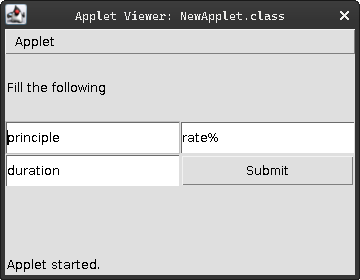
\includegraphics[width=0.4\textwidth]{./assets/p17-s1.png}
	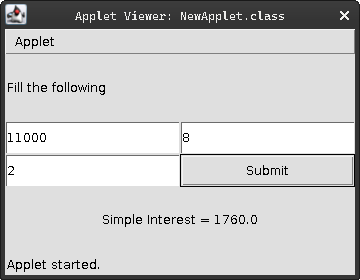
\includegraphics[width=0.4\textwidth]{./assets/p17-s2.png}
\end{figure}

\end{document}
